\documentclass[11pt,a4paper]{article}
\usepackage[utf8]{inputenc}
\usepackage[T1]{fontenc}
\usepackage{lmodern}
\usepackage{amsmath,amssymb,mathtools}
\usepackage[margin=2.2cm]{geometry}
\usepackage{microtype}
\usepackage{booktabs,array,tabularx}
\usepackage{enumitem}
\usepackage{xcolor}
\usepackage[most]{tcolorbox}
\usepackage[colorlinks=true,linkcolor=blue!60!black,urlcolor=blue!60!black]{hyperref}
\usepackage{fancyhdr}
\usepackage{tikz}
\usetikzlibrary{positioning}
\setlength{\parindent}{0pt}
\setlength{\parskip}{6pt}
\renewcommand{\arraystretch}{1.25}
\pagestyle{fancy}
\fancyhf{}
\fancyhead[L]{\small GATE DA 2027 --- Linear Algebra}
\fancyhead[R]{\small Ramu \& Somu Notes}
\fancyfoot[C]{\thepage}

% ---------- macros ----------
\newcommand{\T}{^{\top}}
\newcommand{\R}{\mathbb{R}}
\newcommand{\rank}{\operatorname{rank}}
\newcommand{\nullity}{\operatorname{nullity}}
\newcommand{\tr}{\operatorname{tr}}
\newcommand{\diag}{\operatorname{diag}}
\newcommand{\spn}{\operatorname{span}}
\newcommand{\Null}{\mathcal{N}}
\newcommand{\Col}{\mathcal{C}}
\newcommand{\vecc}[1]{\begin{pmatrix}#1\end{pmatrix}}

% ---------- boxes ----------
\newtcolorbox{story}[1][]{breakable,enhanced,colback=yellow!10,colframe=orange!80!black,
  fonttitle=\bfseries,title={Ramu \& Somu: #1},left=6pt,right=6pt,top=4pt,bottom=4pt}
\newtcolorbox{formula}[1][Formulas]{breakable,enhanced,colback=blue!5,colframe=blue!60!black,
  fonttitle=\bfseries,title={#1},left=6pt,right=6pt}
\newtcolorbox{example}[1][Worked example]{breakable,enhanced,colback=green!6,colframe=green!45!black,
  fonttitle=\bfseries,title={#1},left=6pt,right=6pt}
\newtcolorbox{trap}{breakable,enhanced,colback=red!5,colframe=red!60!black,
  fonttitle=\bfseries,title={Common GATE traps},left=6pt,right=6pt}
\newtcolorbox{intuition}{breakable,enhanced,colback=gray!8,colframe=gray!60!black,
  fonttitle=\bfseries,title={Idea in plain words},left=6pt,right=6pt}

\title{\Huge\bfseries GATE DA 2027\\[4pt] \Large Linear Algebra --- Deep Edition\\[8pt]
\large Vector spaces, matrices, systems, eigenvalues, quadratic forms, LU and SVD,\\ with all GATE DA 2024--2026 questions solved and connected,\\ told by Ramu and Somu}
\author{}
\date{}

\begin{document}
\maketitle
\thispagestyle{empty}

\begin{center}
\begin{tcolorbox}[colback=yellow!10,colframe=orange!80!black,width=0.9\textwidth,breakable]
\textbf{The two friends are back.}\\
\textbf{Ramu} asks ``but why?'' about everything. \textbf{Somu} explains with small everyday examples. Linear algebra is the maths of \emph{many numbers at once}, so most of our stories are about bags of fruit, shops, and a small town's roads.\\[4pt]
\textbf{How the book is organised:} \textbf{Part I} teaches every topic. \textbf{Part II} solves all $19$ Linear Algebra questions from GATE DA 2024, 2025 and 2026 and connects each to its topic. \textbf{Part III} gives proofs and deeper explanations. Answers are checked against the official keys and by computation.\\[4pt]
\textbf{Syllabus covered (GATE DA, Section 2):} vector spaces, matrix types, quadratic forms, linear systems, eigenvalues and eigenvectors, rank and nullity, LU decomposition and SVD.
\end{tcolorbox}
\end{center}

\tableofcontents
\newpage

% =====================================================================
\part{Core Notes: Topic by Topic}
\section{Vectors and Vector Spaces}

\begin{story}[Fruit shopping lists]
Ramu goes to the market and buys \textbf{2 apples and 3 bananas}. Somu writes this as a vector $\vecc{2\\3}$. Another day Ramu buys $\vecc{1\\0}$ (one apple) and $\vecc{0\\1}$ (one banana). Any shopping list can be built from these two: $\vecc{2\\3}=2\vecc{1\\0}+3\vecc{0\\1}$. This is a \textbf{linear combination}, and the two basic lists form a \textbf{basis} for the ``fruit space'' $\R^2$.

But if Ramu is given the lists $\vecc{1\\2}$ and $\vecc{2\\4}$, the second is just double the first. No matter how he combines them, he can only produce lists along one line. They are \textbf{linearly dependent}: one of them is wasted.
\end{story}

\subsection{Vector space and subspace}
\begin{formula}[Definitions]
A \textbf{vector space} over $\R$ is a set closed under addition and scalar multiplication (with the usual axioms: zero vector, additive inverse, associativity, distributivity, etc.).\\[2pt]
A \textbf{subspace} $W\subseteq V$ must satisfy: (i) $0\in W$; (ii) $u,v\in W\Rightarrow u+v\in W$; (iii) $u\in W,\ c\in\R\Rightarrow cu\in W$.\\[2pt]
Examples of subspaces of $\R^n$: the zero set $\{0\}$, lines and planes through the origin, the solution set of $A\mathbf{x}=\mathbf 0$, the column space of any matrix. \textbf{Non-examples:} a line not through $0$; the set $\{x: x\ge0\}$ (not closed under negatives).
\end{formula}

\subsection{Span, independence, basis, dimension}
\begin{formula}
\begin{itemize}[leftmargin=1.2em,itemsep=3pt,topsep=2pt]
\item Linear combination:  $c_1v_1+c_2v_2+\cdots+c_kv_k$
\item $\spn\{v_1,\dots,v_k\}=$  set of all linear combinations (a subspace)
\item Linearly independent:  $c_1v_1+\cdots+c_kv_k=0\ \Rightarrow\ c_1=\cdots=c_k=0$
\item Basis:  linearly independent \emph{and} spans  $V$
\item $\dim V=$  number of vectors in any basis (all bases have the same size)
\item $\dim\R^n=n,\qquad \dim($ space of  $m\times n$  matrices $)=mn,\qquad \dim($ polynomials of degree $\le d)=d+1$
\end{itemize}
\end{formula}

\begin{intuition}
Independence means \emph{no vector is redundant}. Practical test: put the vectors as columns of a matrix $A$. They are independent exactly when $A\mathbf c=\mathbf 0$ has only the solution $\mathbf c=\mathbf 0$, i.e.\ when $\rank(A)$ equals the number of vectors. In $\R^n$, any set of more than $n$ vectors is dependent; any $n$ independent vectors form a basis.
\end{intuition}

\begin{example}[Independent or not?]
$v_1=(1,2,3)$, $v_2=(2,4,6)$, $v_3=(1,0,1)$. Since $v_2=2v_1$, the set is dependent. $\spn\{v_1,v_2,v_3\}=\spn\{v_1,v_3\}$ has dimension $2$ (a plane in $\R^3$).
\end{example}

\subsection{The four fundamental subspaces}
\begin{story}[A shop's price list]
Somu runs a small stall with a matrix $A$ ($m\times n$): each row is a customer and each column an item. Ramu asks about four natural questions:
\begin{itemize}[noitemsep]
\item Which totals $\mathbf b$ can the stall produce? $\Rightarrow$ the \textbf{column space}.
\item Which combinations of items give a zero bill? $\Rightarrow$ the \textbf{null space}.
\end{itemize}
Row space and left null space are the same two questions for $A\T$.
\end{story}
\begin{formula}
For an $m\times n$ matrix $A$ with $\rank(A)=r$:
\begin{center}
\begin{tabular}{llll}
\toprule
\textbf{Subspace} & \textbf{Lives in} & \textbf{Dimension} & \textbf{Meaning}\\
\midrule
Column space $\Col(A)$ & $\R^m$ & $r$ & all $A\mathbf x$\\
Null space $\Null(A)$ & $\R^n$ & $n-r$ & all $\mathbf x$ with $A\mathbf x=0$\\
Row space $\Col(A\T)$ & $\R^n$ & $r$ & span of rows\\
Left null space $\Null(A\T)$ & $\R^m$ & $m-r$ & all $\mathbf y$ with $A\T\mathbf y=0$\\
\bottomrule
\end{tabular}
\end{center}
Orthogonality: row space $\perp$ null space (in $\R^n$); column space $\perp$ left null space (in $\R^m$).
\end{formula}

\subsection{Inner product, norm, orthogonality, projection}
\begin{formula}
\begin{align*}
&\langle u,v\rangle=u\T v=\sum u_iv_i,\qquad \|u\|=\sqrt{u\T u},\qquad \cos\theta=\frac{u\T v}{\|u\|\|v\|}\\
&\text{Cauchy--Schwarz: }|u\T v|\le\|u\|\|v\|,\qquad \text{Triangle: }\|u+v\|\le\|u\|+\|v\|\\
&u\perp v\iff u\T v=0\qquad(\text{orthogonal nonzero vectors are independent})\\
&\text{Projection of } b \text{ onto } a:\quad \operatorname{proj}_a b=\frac{a\T b}{a\T a}\,a,\qquad P=\frac{aa\T}{a\T a}\\
&\text{Projection onto }\Col(A)\ (A\text{ full column rank}):\quad P=A(A\T A)^{-1}A\T\\
&\text{Least squares: minimise }\|Ax-b\|^2\ \Rightarrow\ \text{normal equations }A\T A\,\hat x=A\T b
\end{align*}
\end{formula}

\begin{story}[Making directions perpendicular: Gram--Schmidt]
Ramu has two directions $v_1=(1,1,0)$ and $v_2=(1,0,1)$ and wants a pair of \emph{perpendicular unit} directions covering the same plane. Somu: keep the first direction, then remove from the second whatever lies along the first.
\[
e_1=\frac{v_1}{\|v_1\|}=\frac{1}{\sqrt2}(1,1,0),\qquad
w_2=v_2-(v_2\T e_1)e_1=(1,0,1)-\tfrac12(1,1,0)=\big(\tfrac12,-\tfrac12,1\big),
\]
\[
e_2=\frac{w_2}{\|w_2\|}=\frac{1}{\sqrt{3/2}}\big(\tfrac12,-\tfrac12,1\big).
\]
Check $e_1\T e_2\propto\tfrac12-\tfrac12=0$. This is the \textbf{Gram--Schmidt process}, giving $A=QR$ ($Q$ orthonormal columns, $R$ upper triangular).
\end{story}

\begin{trap}
(1) A subspace must contain $0$. (2) Dependent vectors can still span (they just contain redundancy). (3) $\dim$ of the solution set of $A\mathbf x=\mathbf b$ ($\mathbf b\neq0$) is not a vector-space dimension in the same sense: it is a \emph{shifted} subspace (an affine set) with the same ``size'' $n-r$.
\end{trap}

% =====================================================================
\newpage
\section{Matrix Types and Basic Operations}

\begin{story}[A town's roads]
Somu draws a map of 3 villages and writes a $3\times3$ matrix where entry $(i,j)$ is $1$ if there is a road from village $i$ to $j$. Ramu notices: if all roads are two-way, the matrix equals its own mirror image across the diagonal. Such a matrix is \textbf{symmetric}. Different shapes of matrix tell us different stories, and each has a name.
\end{story}

\subsection{Catalogue of special matrices}
\begin{center}
\small
\begin{tabularx}{\textwidth}{>{\raggedright\arraybackslash}p{3.0cm} >{\raggedright\arraybackslash}p{4.4cm} >{\raggedright\arraybackslash}X}
\toprule
\textbf{Type} & \textbf{Definition} & \textbf{Key facts}\\
\midrule
Diagonal & $a_{ij}=0$ for $i\ne j$ & eigenvalues = diagonal entries; $\det=\prod d_i$\\
Identity $I$ & diagonal with 1's & $AI=IA=A$\\
Upper / lower triangular & zeros below / above diagonal & eigenvalues = diagonal entries; $\det=\prod$ diagonal\\
Symmetric & $A\T=A$ & real eigenvalues; orthogonal eigenvectors; diagonalisable\\
Skew-symmetric & $A\T=-A$ & diagonal $=0$; eigenvalues purely imaginary or $0$; odd order $\Rightarrow\det=0$\\
Orthogonal & $Q\T Q=QQ\T=I$ & $Q^{-1}=Q\T$; $\det=\pm1$; $|\lambda|=1$; preserves lengths\\
Idempotent & $A^2=A$ & eigenvalues $0$ or $1$; projections\\
Nilpotent & $A^k=0$ for some $k$ & all eigenvalues $0$\\
Involutory & $A^2=I$ & eigenvalues $\pm1$\\
Singular & $\det A=0$ & not invertible; has eigenvalue $0$; $\rank<n$\\
Invertible (non-singular) & $\det A\ne0$ & $\rank=n$; unique solution to $A\mathbf x=\mathbf b$\\
Positive definite & symmetric, $x\T Ax>0\ \forall x\ne0$ & all eigenvalues $>0$ (see Section~\ref{sec:quad})\\
Hermitian (complex) & $A^*=A$ & real eigenvalues\\
Unitary (complex) & $U^*U=I$ & complex analogue of orthogonal\\
\bottomrule
\end{tabularx}
\end{center}

\subsection{Rules of matrix arithmetic}
\begin{formula}
\begin{align*}
&(AB)\T=B\T A\T,\qquad (AB)^{-1}=B^{-1}A^{-1},\qquad (A\T)^{-1}=(A^{-1})\T\\
&AB\ne BA\ \text{in general};\quad (A+B)^2\ne A^2+2AB+B^2\ \text{unless }AB=BA\\
&\tr(A)=\sum a_{ii},\qquad \tr(AB)=\tr(BA),\qquad \tr(A+B)=\tr A+\tr B\\
&\text{Any square }A=\underbrace{\tfrac12(A+A\T)}_{\text{symmetric}}+\underbrace{\tfrac12(A-A\T)}_{\text{skew-symmetric}}\\
&2\times2\text{ inverse: }\begin{pmatrix}a&b\\c&d\end{pmatrix}^{-1}=\frac{1}{ad-bc}\begin{pmatrix}d&-b\\-c&a\end{pmatrix}\\
&A^{-1}=\frac{\operatorname{adj}(A)}{\det A},\qquad \operatorname{adj}(A)=\text{transpose of the cofactor matrix}
\end{align*}
\end{formula}

\subsection{Determinant}
\begin{formula}
\begin{itemize}[leftmargin=1.2em,itemsep=3pt,topsep=2pt]
\item $\det\begin{pmatrix}a&b\\c&d\end{pmatrix}=ad-bc$
\item $\det(AB)=\det A\det B,\qquad \det(A\T)=\det A,\qquad \det(A^{-1})=\frac1{\det A}$
\item $\det(cA)=c^n\det A\ \ (n\times n),\qquad \det(A^k)=(\det A)^k$
\item Row swap: $\det\to-\det$; scale a row by $c$: $\det\to c\det$; add a multiple of one row to another: $\det$ unchanged.
\item Two equal (or proportional) rows or a zero row  $\Rightarrow\det=0$
\item $\det A=\prod_i\lambda_i,\qquad \tr A=\sum_i\lambda_i\qquad($ eigenvalues with multiplicity $)$
\end{itemize}
\end{formula}

\begin{example}
$A=\begin{pmatrix}1&2\\3&4\end{pmatrix}$: $\det A=4-6=-2$, $\det(2A)=2^2(-2)=-8$, $A^{-1}=\frac{1}{-2}\begin{pmatrix}4&-2\\-3&1\end{pmatrix}=\begin{pmatrix}-2&1\\1.5&-0.5\end{pmatrix}$.
\end{example}

% =====================================================================
\newpage
\section{Linear Systems $A\mathbf x=\mathbf b$}

\begin{story}[Ramu's three shops]
Ramu buys 3 kinds of fruit from a stall but forgets the prices. He remembers three bills:
\[
x+y+z=6,\qquad 2y+5z=-4,\qquad 2x+5y-z=27 .
\]
(Here the numbers are just for practice.) Somu solves it by \textbf{Gaussian elimination}: use the first equation to remove $x$ from the others, then use the next to remove $y$, then back-substitute. Result: $x=5,\ y=3,\ z=-2$. Check: $5+3-2=6$, $6-10=-4$, $10+15+2=27$.
\end{story}

\subsection{Matrix form and elimination}
\begin{formula}
\begin{itemize}[leftmargin=1.2em,itemsep=3pt,topsep=2pt]
\item $A\mathbf x=\mathbf b,\quad A\in\R^{m\times n}\ (m$  equations $,\ n$  unknowns $),$ augmented matrix  $[A\mid\mathbf b]$
\item Row operations: swap rows; scale a row; add a multiple of one row to another (do not change the solution set)
\item Gauss elimination $\to$ row echelon form \hspace{0.8em} Gauss--Jordan $\to$ reduced row echelon form (RREF)
\item Pivot columns  $\leftrightarrow$  basic variables;\quad non-pivot columns  $\leftrightarrow$  free variables
\end{itemize}
\end{formula}

\subsection{When does a solution exist? (The master table)}
\begin{formula}[Rouch\'e--Capelli theorem]
Let $r=\rank(A)$, $r_{aug}=\rank([A\mid\mathbf b])$, $n=$ number of unknowns.
\begin{center}
\begin{tabular}{lll}
\toprule
\textbf{Condition} & \textbf{Result} & \textbf{Free variables}\\
\midrule
$r<r_{aug}$ & \textbf{no solution} (inconsistent) & ---\\
$r=r_{aug}=n$ & \textbf{unique solution} & $0$\\
$r=r_{aug}<n$ & \textbf{infinitely many solutions} & $n-r$\\
\bottomrule
\end{tabular}
\end{center}
Always $r\le r_{aug}\le r+1$.
\end{formula}

\subsection{Homogeneous systems $A\mathbf x=\mathbf 0$}
\begin{formula}
\begin{itemize}[noitemsep]
\item Always consistent (the zero solution). It has a \textbf{non-trivial} solution $\iff r<n$.
\item If $m<n$ (fewer equations than unknowns), there are always non-trivial solutions.
\item For square $A$: non-trivial solution $\iff\det A=0$.
\item Solution set $=\Null(A)$, a subspace of dimension $n-r$.
\item General solution of $A\mathbf x=\mathbf b$: $\ \mathbf x=\mathbf x_p+\mathbf x_h$ (one particular solution plus anything in the null space).
\end{itemize}
Cramer's rule (square, $\det A\ne0$): $\ x_i=\dfrac{\det A_i}{\det A}$, where $A_i$ is $A$ with column $i$ replaced by $\mathbf b$.
\end{formula}

\begin{example}[Inconsistent vs infinite]
$x+y=2,\ x+y=3$: $r=1$, $r_{aug}=2$, \textbf{no solution} (parallel lines).\\
$x+y=2,\ 2x+2y=4$: $r=r_{aug}=1<2$, so \textbf{infinitely many} (1 free variable): $(2-t,\ t)$.\\
Three equations, five unknowns, $\rank=3$: $5-3=2$ free variables, infinitely many solutions.
\end{example}

\begin{trap}
(1) Comparing only $\rank(A)$ with $n$ is not enough; \emph{always compare with $\rank[A|\mathbf b]$}. (2) A square system with $\det A=0$ can have either no solution or infinitely many. (3) ``Free variables $=n-\rank$'' counts unknowns, not equations.
\end{trap}

% =====================================================================
\newpage
\section{Rank and Nullity}

\begin{story}[Duplicate shopkeepers]
Somu has a table of 4 shopkeepers' price lists (4 rows). But two of the shopkeepers simply copy each other, and the fourth always quotes exactly the sum of the other two. Ramu asks, ``How many \emph{truly different} shopkeepers are there?'' The answer is the \textbf{rank}: the number of independent rows (equivalently, independent columns). A rank-deficient matrix hides redundancy.
\end{story}

\begin{formula}
\begin{itemize}[leftmargin=1.2em,itemsep=3pt,topsep=2pt]
\item $\rank(A)=$ number of pivots $=\dim\Col(A)=\dim($ row space $)=$ max number of independent rows (or columns)
\item $\nullity(A)=\dim\Null(A)=n-\rank(A)\qquad(\textbf{Rank--Nullity theorem},\ A\in\R^{m\times n})$
\item $\rank(A)\le\min(m,n),\qquad \rank(A)=\rank(A\T)$
\item $\rank(AB)\le\min(\rank A,\rank B),\qquad \rank(A+B)\le\rank A+\rank B$
\item $\rank(A\T A)=\rank(AA\T)=\rank(A)$
\item Sylvester:  $\rank A+\rank B-n\le\rank(AB)\ \ (A:m\times n,\ B:n\times p)$
\item Square  $A:$ invertible $\iff\rank=n\iff\det\ne0\iff$ columns independent $\iff0$  is not an eigenvalue
\item Rank-1 matrix:  $A=uv\T\ ($ outer product $)\ \Rightarrow\ \rank=1,$ only nonzero eigenvalue  $v\T u$
\end{itemize}
\end{formula}

\begin{example}
$A=\begin{pmatrix}1&2&3\\2&4&6\\1&0&1\end{pmatrix}$. Row 2 is $2\times$ row 1, so $\rank A=2$, $\nullity=3-2=1$, $\det A=0$. Null space: $x+2y+3z=0$ and $x+z=0\Rightarrow x=-z,\ y=-z$, i.e.\ spanned by $(-1,-1,1)$. Check: $-1-2+3=0$, $-1+0+1=0$.\\
For a $4\times6$ matrix with $\rank=3$: $\nullity=6-3=3$; left null space has dimension $4-3=1$.
\end{example}

\begin{trap}
Rank is found by row-reducing but \textbf{row operations do not change the row space or rank}, while they \emph{do} change the column space (its dimension stays the same). $\rank(A+B)$ is only bounded, not equal to the sum.
\end{trap}

% =====================================================================
\newpage
\section{Eigenvalues and Eigenvectors}

\begin{story}[A machine that only stretches]
Ramu has a machine that transforms points of the plane: $\mathbf x\mapsto A\mathbf x$. For most arrows the machine \emph{turns and stretches} them. But Somu finds special arrows that the machine only \emph{stretches} without turning: $A\mathbf v=\lambda\mathbf v$. These are \textbf{eigenvectors}, and the stretch factors $\lambda$ are \textbf{eigenvalues}. (``Eigen'' means ``own'' in German: the matrix's own special directions.)
\end{story}

\subsection{Definition and how to compute}
\begin{formula}
\begin{align*}
&A\mathbf v=\lambda\mathbf v,\quad\mathbf v\ne0\iff(A-\lambda I)\mathbf v=0\text{ has a nonzero solution}\iff\det(A-\lambda I)=0\\
&\text{Characteristic polynomial: }p(\lambda)=\det(\lambda I-A)=\lambda^n-(\tr A)\lambda^{n-1}+\cdots+(-1)^n\det A\\
&\text{For }2\times2:\ \lambda^2-(\tr A)\lambda+\det A=0\\
&\text{Eigenvectors for }\lambda:\ \text{non-zero vectors in }\Null(A-\lambda I)\ (\text{the eigenspace})
\end{align*}
\end{formula}

\subsection{Properties you must know}
\begin{formula}
\begin{align*}
&\sum\lambda_i=\tr A,\qquad \prod\lambda_i=\det A\\
&\text{Eigenvalues of }A^k:\ \lambda^k;\quad A^{-1}:\ 1/\lambda;\quad A+cI:\ \lambda+c;\quad cA:\ c\lambda;\quad p(A):\ p(\lambda)\\
&A\text{ and }A\T\text{ have the same eigenvalues (not the same eigenvectors)}\\
&AB\text{ and }BA\text{ have the same nonzero eigenvalues}\\
&\text{Triangular/diagonal: eigenvalues are the diagonal entries}\\
&\text{Eigenvectors for \emph{distinct} eigenvalues are linearly independent}\\
&\text{Symmetric real }A:\ \text{real eigenvalues; eigenvectors for distinct eigenvalues are orthogonal}\\
&\text{Singular}\iff 0\text{ is an eigenvalue};\quad\text{Idempotent: }\lambda\in\{0,1\};\quad\text{Orthogonal: }|\lambda|=1\\
&\text{Cayley--Hamilton: }p(A)=0\ (\text{every matrix satisfies its own characteristic equation})
\end{align*}
\end{formula}

\subsection{Multiplicities and diagonalisation}
\begin{formula}
\begin{itemize}[leftmargin=1.2em,itemsep=3pt,topsep=2pt]
\item Algebraic multiplicity (AM) $=$ multiplicity of  $\lambda$  as a root of  $p(\lambda)$
\item Geometric multiplicity (GM) $=\dim\Null(A-\lambda I),\qquad 1\le\mathrm{GM}\le\mathrm{AM}$
\item $A$  is \textbf{diagonalisable} $\iff\mathrm{GM}=\mathrm{AM}$  for every eigenvalue $\iff A$  has  $n$  independent eigenvectors
\item Then  $A=PDP^{-1},\ D=\diag(\lambda_1,\dots,\lambda_n),\ P=[\mathbf v_1\ \cdots\ \mathbf v_n],\quad A^k=PD^kP^{-1}$
\item Symmetric  $A=Q\Lambda Q\T\ ($ spectral theorem,  $Q$  orthogonal $)$
\end{itemize}
\end{formula}

\begin{story}[Powers of a machine]
Ramu applies the machine $A=\begin{pmatrix}4&1\\2&3\end{pmatrix}$ to a point 10 times. Multiplying matrices 10 times is painful, so Somu finds the eigenvalues: $\tr A=7$, $\det A=10$, so $\lambda^2-7\lambda+10=0\Rightarrow\lambda=5,2$.\\
For $\lambda=5$: $(A-5I)=\begin{pmatrix}-1&1\\2&-2\end{pmatrix}\Rightarrow\mathbf v_1=(1,1)$.\\
For $\lambda=2$: $(A-2I)=\begin{pmatrix}2&1\\2&1\end{pmatrix}\Rightarrow\mathbf v_2=(1,-2)$.\\
Check: $A(1,-2)=(4-2,\ 2-6)=(2,-4)=2(1,-2)$. \checkmark\\
So $A=PDP^{-1}$ with $P=\begin{pmatrix}1&1\\1&-2\end{pmatrix}$, $D=\diag(5,2)$, and $A^{10}=P\diag(5^{10},2^{10})P^{-1}$: just raise two numbers to the 10th power. In the direction $\mathbf v_1$ everything grows by 5 each step; in $\mathbf v_2$ by 2. Cayley--Hamilton check: $A^2-7A+10I=\begin{pmatrix}18&7\\14&11\end{pmatrix}-\begin{pmatrix}28&7\\14&21\end{pmatrix}+\begin{pmatrix}10&0\\0&10\end{pmatrix}=0$.
\end{story}

\begin{example}[Not diagonalisable]
$A=\begin{pmatrix}1&1\\0&1\end{pmatrix}$: $\lambda=1$ twice (AM $=2$), but $A-I=\begin{pmatrix}0&1\\0&0\end{pmatrix}$ has nullity $1$ (GM $=1$). Only one independent eigenvector, so \textbf{not} diagonalisable.\\
Given eigenvalues $1,2,3$: $\det A=6$, $\tr A=6$; $A^2$ has $1,4,9$ ($\tr A^2=14$); $A^{-1}$ has $1,\frac12,\frac13$; $A+2I$ has $3,4,5$.
\end{example}

\begin{trap}
(1) Repeated eigenvalues do \emph{not} automatically mean non-diagonalisable (e.g.\ $I$), but check GM vs AM. (2) Eigenvectors for the \emph{same} eigenvalue are not necessarily orthogonal, only for distinct eigenvalues of a symmetric matrix. (3) $\tr$ and $\det$ give quick checks on your eigenvalue computation: always verify.
\end{trap}

% =====================================================================
\newpage
\section{Quadratic Forms and Definiteness}\label{sec:quad}

\begin{story}[The shape of a bowl]
Somu holds a quadratic function $q(x,y)=2x^2+2xy+2y^2$ and asks Ramu, ``If I plot this, what shape do I get?'' Ramu guesses a bowl: it is non-negative and zero only at the origin. Somu writes $q$ with a \textbf{symmetric matrix}: $q=\mathbf x\T A\mathbf x$ with $A=\begin{pmatrix}2&1\\1&2\end{pmatrix}$. The matrix tells him the shape: eigenvalues $3$ and $1$ are both positive, so it is a bowl opening upward in every direction (\textbf{positive definite}). If one eigenvalue were negative, the surface would be a saddle.
\end{story}

\subsection{Definitions}
\begin{formula}
A \textbf{quadratic form} in $\mathbf x\in\R^n$: $\ q(\mathbf x)=\mathbf x\T A\mathbf x=\sum_{i,j}a_{ij}x_ix_j$, with $A$ taken \textbf{symmetric}. (A non-symmetric $B$ gives the same form as $\tfrac12(B+B\T)$.)\\[3pt]
To get $A$: diagonal entries $=$ coefficients of $x_i^2$; off-diagonal $a_{ij}=a_{ji}=\tfrac12\times$ (coefficient of $x_ix_j$).
\end{formula}

\begin{center}
\begin{tabularx}{\textwidth}{>{\raggedright\arraybackslash}p{3.6cm} >{\raggedright\arraybackslash}p{4.4cm} >{\raggedright\arraybackslash}X}
\toprule
\textbf{Name} & \textbf{Condition on }$\mathbf x\T A\mathbf x$ & \textbf{Eigenvalues of symmetric }$A$\\
\midrule
Positive definite (PD) & $>0$ for all $\mathbf x\ne0$ & all $>0$\\
Positive semidefinite (PSD) & $\ge0$ for all $\mathbf x$ & all $\ge0$\\
Negative definite (ND) & $<0$ for all $\mathbf x\ne0$ & all $<0$\\
Negative semidefinite & $\le0$ & all $\le0$\\
Indefinite & takes both signs & both positive and negative\\
\bottomrule
\end{tabularx}
\end{center}

\subsection{Tests for definiteness}
\begin{formula}
\begin{itemize}[noitemsep]
\item \textbf{Eigenvalue test:} signs of the eigenvalues (above).
\item \textbf{Sylvester's criterion:} $A$ is PD $\iff$ all \emph{leading principal minors} $\Delta_1,\Delta_2,\dots,\Delta_n>0$. $A$ is ND $\iff$ signs alternate $\Delta_1<0,\Delta_2>0,\Delta_3<0,\dots$
\item \textbf{PSD needs \emph{all} principal minors} $\ge0$ (not just the leading ones).
\item $2\times2$: PD $\iff a>0$ and $ad-b^2>0$ (equivalently $\tr>0$ and $\det>0$).
\item $B\T B$ is always PSD; PD iff $B$ has full column rank. Also $A$ PD $\Rightarrow$ $A$ invertible, $a_{ii}>0$.
\item \textbf{Diagonalising a form:} with $A=Q\Lambda Q\T$ and $\mathbf y=Q\T\mathbf x$: $q=\sum\lambda_iy_i^2$. \textbf{Rank} of the form $=$ rank of $A$; \textbf{signature} $=$ (\#positive) $-$ (\#negative) eigenvalues. (Sylvester's law of inertia.)
\item Link to calculus: the Hessian $H$ at a critical point: PD $\Rightarrow$ local minimum, ND $\Rightarrow$ local maximum, indefinite $\Rightarrow$ saddle.
\item \textbf{Rayleigh quotient:} $\lambda_{\min}\le\dfrac{\mathbf x\T A\mathbf x}{\mathbf x\T\mathbf x}\le\lambda_{\max}$ for symmetric $A$.
\end{itemize}
\end{formula}

\begin{example}
$A=\begin{pmatrix}2&-1&0\\-1&2&-1\\0&-1&2\end{pmatrix}$: leading minors $2,\ 3,\ 4$ are all positive, so $A$ is \textbf{PD}. (Eigenvalues $2,\ 2\pm\sqrt2$, all positive; sum $=6=\tr A$, product $=4=\det A$.)\\
$\begin{pmatrix}1&2\\2&1\end{pmatrix}$: $\det=1-4=-3<0$, eigenvalues $3,-1$: \textbf{indefinite}.\\
$q=x^2+4xy+y^2$ has matrix $\begin{pmatrix}1&2\\2&1\end{pmatrix}$ (the $xy$ coefficient $4$ is split as $2+2$): indefinite.
\end{example}

\begin{trap}
(1) Always symmetrise first. (2) Positive determinant alone does not imply PD: $\begin{pmatrix}-1&0\\0&-1\end{pmatrix}$ has $\det=1$ but is ND. (3) Sylvester's test for \emph{semi}definiteness needs all principal minors, not just leading ones.
\end{trap}

% =====================================================================
\newpage
\section{LU Decomposition}

\begin{story}[Solving the same problem for many customers]
Somu's stall has a fixed price matrix $A$ but every day a different bill vector $\mathbf b$. Doing full elimination every day would be wasteful. Instead, Somu does the elimination \emph{once}, records the steps in a matrix $L$ and keeps the result in $U$. Now each new day costs only two cheap back-substitutions. That is LU decomposition: $A=LU$.
\end{story}

\begin{formula}
\begin{itemize}[leftmargin=1.2em,itemsep=3pt,topsep=2pt]
\item $A=LU:\ L$  lower triangular with ones on the diagonal (stores the multipliers) $,\ U$  upper triangular (the echelon form)
\item Solving  $A\mathbf x=\mathbf b:\quad L\mathbf y=\mathbf b\ ($ forward substitution $),\quad U\mathbf x=\mathbf y\ ($ back substitution $)$
\item $\det A=\det U=\prod u_{ii}\qquad(\det L=1)$
\item If a zero (or tiny) pivot appears, swap rows:  $PA=LU\ (P=$ permutation matrix $,\ \det P=\pm1)$
\item Multiplier: $\ell_{ij}=\dfrac{a_{ij}}{a_{jj}}$ evaluated on the current (partly reduced) matrix. You do $R_i\leftarrow R_i-\ell_{ij}R_j$, and $L$ stores $\ell_{ij}$.
\item Cost: elimination  $\sim\tfrac23n^3$  operations; each extra  $\mathbf b$  costs only  $\sim2n^2$
\item Symmetric positive definite  $A:$ Cholesky  $A=LL\T\ ($ half the cost $),\quad A=LDL\T$
\end{itemize}
\end{formula}

\begin{example}[A full LU example]
$A=\begin{pmatrix}2&1&1\\4&3&3\\8&7&9\end{pmatrix}$.\\
\textbf{Step 1} (pivot $2$): $R_2\leftarrow R_2-2R_1$ ($\ell_{21}=2$), $R_3\leftarrow R_3-4R_1$ ($\ell_{31}=4$):
$\begin{pmatrix}2&1&1\\0&1&1\\0&3&5\end{pmatrix}$.\\
\textbf{Step 2} (pivot $1$): $R_3\leftarrow R_3-3R_2$ ($\ell_{32}=3$): $U=\begin{pmatrix}2&1&1\\0&1&1\\0&0&2\end{pmatrix}$.\\
Hence
\[
L=\begin{pmatrix}1&0&0\\2&1&0\\4&3&1\end{pmatrix},\qquad
U=\begin{pmatrix}2&1&1\\0&1&1\\0&0&2\end{pmatrix},\qquad LU=A .
\]
\textbf{Determinant:} $\det A=2\cdot1\cdot2=4$.\\
\textbf{Solve} $A\mathbf x=\mathbf b$ with $\mathbf b=(4,10,24)$: forward: $y_1=4$, $y_2=10-2(4)=2$, $y_3=24-4(4)-3(2)=2$. Back: $x_3=2/2=1$, $x_2=2-1=1$, $x_1=(4-1-1)/2=1$. So $\mathbf x=(1,1,1)$. \checkmark
\end{example}

\begin{trap}
(1) The multipliers go into $L$ with a \emph{positive} sign (you subtract $\ell_{ij}\times$row, so $L$ stores $+\ell_{ij}$). (2) Without row swaps LU exists only if all leading principal minors are nonzero. (3) $\det A=\prod u_{ii}$ only when no row swaps happened; with swaps multiply by $(-1)^{\#\text{swaps}}$.
\end{trap}

% =====================================================================
\newpage
\section{Singular Value Decomposition (SVD)}

\begin{story}[Every matrix is a rotate--stretch--rotate]
Ramu: ``Eigen-decomposition only works for square, nice matrices. What about a $2\times3$ table of ratings?'' Somu: SVD works for \emph{every} matrix. Any linear map can be seen as three simple steps: (1) rotate/reflect the input space ($V\T$), (2) stretch along the coordinate axes by non-negative numbers $\sigma_i$ ($\Sigma$), (3) rotate/reflect in the output space ($U$). The stretch factors $\sigma_i$ are the \textbf{singular values}: how strongly the matrix acts in each of its principal directions.
\end{story}

\begin{formula}
\begin{itemize}[leftmargin=1.2em,itemsep=3pt,topsep=2pt]
\item $A=U\Sigma V\T,\qquad A\in\R^{m\times n},\quad U\in\R^{m\times m}$  orthogonal $,\ V\in\R^{n\times n}$  orthogonal
\item $\Sigma\in\R^{m\times n}$  is ``diagonal'' with  $\sigma_1\ge\sigma_2\ge\cdots\ge\sigma_r>0$  and zeros elsewhere $,\quad r=\rank A$
\item $\sigma_i=\sqrt{\lambda_i(A\T A)}=\sqrt{\lambda_i(AA\T)}\qquad($ non-zero eigenvalues of  $A\T A$  and  $AA\T$  coincide $)$
\item $V:$ eigenvectors of  $A\T A\ ($ right singular vectors $),\quad U:$ eigenvectors of  $AA\T\ ($ left singular vectors $)$
\item $A\mathbf v_i=\sigma_i\mathbf u_i\ \Rightarrow\ \mathbf u_i=\frac{A\mathbf v_i}{\sigma_i}\qquad(i=1,\dots,r)$
\item Outer-product form:  $A=\sum_{i=1}^{r}\sigma_i\,\mathbf u_i\mathbf v_i\T$
\end{itemize}
\end{formula}

\subsection{What SVD tells you}
\begin{formula}
\begin{itemize}[leftmargin=1.2em,itemsep=3pt,topsep=2pt]
\item $\rank A=\#\{\sigma_i>0\}$
\item $\|A\|_2=\sigma_1\ ($ largest stretch $),\qquad \|A\|_F=\sqrt{\sum\sigma_i^2}=\sqrt{\tr(A\T A)}$
\item Condition number:  $\kappa(A)=\sigma_{\max}/\sigma_{\min}\ ($ square invertible  $A)$
\item $|\det A|=\prod\sigma_i\ ($ square  $A)$
\item Column space  $\Col(A)=\spn\{\mathbf u_1,\dots,\mathbf u_r\};\quad \Null(A)=\spn\{\mathbf v_{r+1},\dots,\mathbf v_n\}$
\item $\textbf{Eckart--Young:}$ best rank- $k$  approximation:  $A_k=\sum_{i=1}^{k}\sigma_i\mathbf u_i\mathbf v_i\T,\quad \|A-A_k\|_2=\sigma_{k+1},\quad\|A-A_k\|_F^2=\sum_{i>k}\sigma_i^2$
\item Pseudo-inverse:  $A^{+}=V\Sigma^{+}U\T\ ($ invert non-zero  $\sigma_i)$ least-squares solution  $\hat{\mathbf x}=A^{+}\mathbf b$
\item Symmetric PSD  $A:$ singular values $=$ eigenvalues \hspace{0.8em} symmetric  $A:\ \sigma_i=|\lambda_i|$
\item PCA: for centred data  $X,$ principal directions $=$ right singular vectors of  $X;$ variance along  $\mathbf v_i=\sigma_i^2/(n-1)$
\end{itemize}
\end{formula}

\begin{example}[A full SVD, step by step]
Let $A=\begin{pmatrix}3&2&2\\2&3&-2\end{pmatrix}$ ($2\times3$).\\
\textbf{Step 1.} $AA\T=\begin{pmatrix}17&8\\8&17\end{pmatrix}$ (check: $9+4+4=17$, $6+6-4=8$). Eigenvalues $17\pm8=25,\ 9$. So \textbf{singular values $\sigma_1=5,\ \sigma_2=3$}, $\rank A=2$.\\
\textbf{Step 2.} Eigenvectors of $AA\T$: $\mathbf u_1=\tfrac1{\sqrt2}(1,1)$ for $25$, $\mathbf u_2=\tfrac1{\sqrt2}(1,-1)$ for $9$.\\
\textbf{Step 3.} $\mathbf v_i=A\T\mathbf u_i/\sigma_i$: $A\T(1,1)=(5,5,0)$, so $\mathbf v_1=\tfrac{1}{\sqrt2}(1,1,0)$; $A\T(1,-1)=(1,-1,4)$, so $\mathbf v_2=\tfrac{1}{3\sqrt2}(1,-1,4)$.\\
\textbf{Step 4.} A third orthonormal $\mathbf v_3\in\Null(A)$: $\mathbf v_3=\tfrac13(-2,2,1)$. Check $A\mathbf v_3=(-6+4+2,\ -4+6-2)=(0,0)$. \checkmark\\
Therefore $A=U\Sigma V\T$ with $\Sigma=\begin{pmatrix}5&0&0\\0&3&0\end{pmatrix}$. Here $\|A\|_2=5$, $\|A\|_F=\sqrt{25+9}=\sqrt{34}$, and the best rank-1 approximation is $5\,\mathbf u_1\mathbf v_1\T=\tfrac52\begin{pmatrix}1&1&0\\1&1&0\end{pmatrix}$.
\end{example}

\begin{story}[Compressing a photo]
Ramu stores a $1000\times1000$ photo as a matrix: a million numbers. Somu does SVD and notices the singular values drop quickly: $\sigma_1,\dots,\sigma_{50}$ are large and the rest tiny. Keeping only the top $50$ terms stores $50\times(1000+1000+1)\approx100{,}000$ numbers (a $10\times$ saving) with very little visible loss. By Eckart--Young no other rank-50 matrix is closer to the original. This is how SVD powers image compression, recommender systems, PCA and noise removal.
\end{story}

\begin{trap}
(1) \textbf{Singular values are not eigenvalues} unless $A$ is symmetric PSD. (2) $\sigma_i\ge0$ always, and they are sorted in decreasing order. (3) The \emph{number} of non-zero singular values equals the rank, and $\Sigma$ has the same shape as $A$ ($m\times n$). (4) Sign choices in $\mathbf u_i,\mathbf v_i$ are not unique but must be consistent: $A\mathbf v_i=\sigma_i\mathbf u_i$.
\end{trap}

% =====================================================================
% =====================================================================
\newpage
\part{Previous-Year Questions: GATE DA 2024, 2025, 2026}

\section{How to Use the Past Papers}

\begin{story}[Ramu asks: which questions come from this chapter?]
Ramu: ``Somu, linear algebra has so many topics. What did the examiners really ask?'' Somu lists every Linear Algebra question from the three GATE DA papers released so far. He solves each one, names the idea behind it, and points to the chapter that teaches it. The pattern turns out to be surprisingly small.
\end{story}

\begin{formula}[Facts from the official papers and answer keys (verified)]
\begin{center}
\begin{tabular}{lccc}
\toprule
 & \textbf{2024} & \textbf{2025} & \textbf{2026}\\\midrule
Linear Algebra questions & 6 & 8 & 5\\
1-mark / 2-mark & 2\,/\,4 & 4\,/\,4 & 2\,/\,3\\
Marks from this section & 10 & 12 & 8\\
\bottomrule
\end{tabular}
\end{center}
\textbf{19 questions} in all. Question numbers: 2024: 13, 35, 47, 48, 49, 61. 2025: 12, 13, 25, 28, 37, 38, 50, 52. 2026: 21, 22, 46, 52, 65. Types: MCQ (one answer), MSQ (one or more answers, no partial credit) and NAT (type a number).\\
\textbf{Source note.} The 2024 and 2026 questions are restated from the official IIT papers, and every answer is the official key's. The official 2025 paper file could not be opened here, so the 2025 wording is restated from a published solution set; its answers agree with the official 2025 key and with my own computations.
\end{formula}

\subsection{Where the 19 questions come from}
\begin{center}
\small
\begin{tabularx}{\textwidth}{>{\raggedright\arraybackslash}p{5.0cm}cX}
\toprule
\textbf{Topic group} & \textbf{Count} & \textbf{Questions (year-Q)}\\\midrule
A. Eigenvalues and eigenvectors & 5 & 24-Q13, Q35; 25-Q13; 26-Q21, Q46\\
B. Vector spaces and subspaces & 3 & 24-Q47; 25-Q25; 26-Q22\\
C. Linear systems, rank, elimination cost & 2 & 24-Q48; 25-Q12\\
D. Projection, idempotent and orthogonal matrices & 5 & 24-Q49; 25-Q37, Q50, Q52; 26-Q52\\
E. Quadratic forms, Gram matrices, Rayleigh quotient & 3 & 25-Q28, Q38; 26-Q65\\
F. SVD & 1 & 24-Q61\\
\bottomrule
\end{tabularx}
\end{center}
\textbf{Reading the pattern.} Almost every question can be answered by reasoning about \emph{eigenvalues}: projections have eigenvalues $0$ and $1$, orthogonal matrices have $|\lambda|=1$, Gram matrices have eigenvalues $\ge0$. GATE rarely wants long arithmetic; it wants you to recognise the \emph{type} of matrix and read the answer from its eigenvalues. The two themes that return again and again are \textbf{projection matrices} (five questions touch them: 24-Q49, 25-Q50, 26-Q52, 26-Q65, 25-Q37) and \textbf{rotations} (24-Q13, 25-Q52, 26-Q21, 26-Q46).

\subsection{The concept map}
\begin{center}
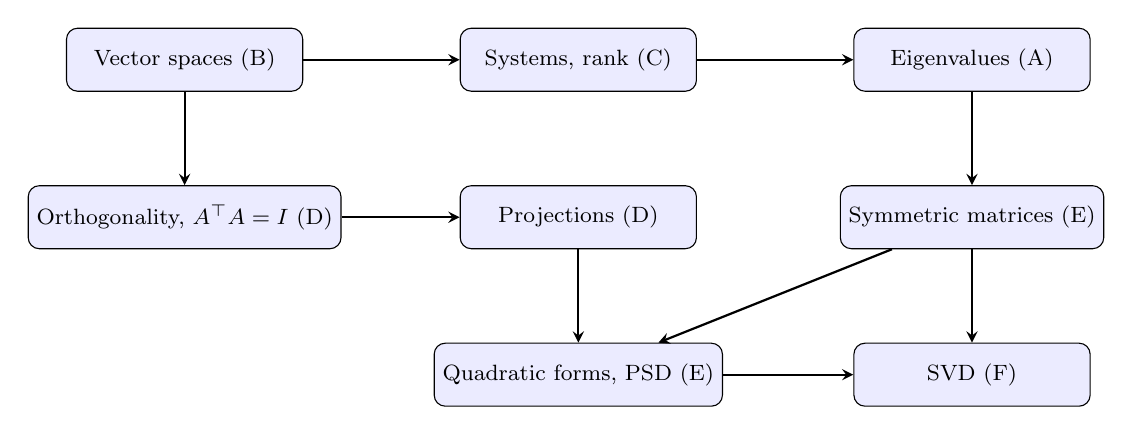
\begin{tikzpicture}[
 b/.style={draw,rounded corners,fill=blue!8,minimum height=8mm,minimum width=30mm,align=center,font=\footnotesize,inner sep=3pt},
 a/.style={->,thick,>=stealth}]
\node[b] (vs) at (0,0) {Vector spaces (B)};
\node[b] (sys) at (5,0) {Systems, rank (C)};
\node[b] (ei) at (10,0) {Eigenvalues (A)};
\node[b] (ort) at (0,-2) {Orthogonality, $A^\top A=I$ (D)};
\node[b] (pro) at (5,-2) {Projections (D)};
\node[b] (sym) at (10,-2) {Symmetric matrices (E)};
\node[b] (qf) at (5,-4) {Quadratic forms, PSD (E)};
\node[b] (svd) at (10,-4) {SVD (F)};
\draw[a](vs)--(sys);\draw[a](sys)--(ei);\draw[a](vs)--(ort);\draw[a](ort)--(pro);
\draw[a](ei)--(sym);\draw[a](pro)--(qf);\draw[a](sym)--(qf);\draw[a](sym)--(svd);\draw[a](qf)--(svd);
\end{tikzpicture}
\end{center}

% =====================================================================
\section{Group A: Eigenvalues and Eigenvectors (5 questions)}

\begin{story}[Look at the trace and the determinant]
Ramu: ``Must I solve a characteristic polynomial every time?'' Somu: ``For a $2\times2$ matrix you only need two numbers: the trace $=\lambda_1+\lambda_2$ and the determinant $=\lambda_1\lambda_2$. They tell you everything: whether the eigenvalues are real, positive, zero, or complex.''
\end{story}

\begin{formula}[Facts used in Group A]
$\sum\lambda_i=\tr A$, \quad $\prod\lambda_i=\det A$. For $2\times2$: $\lambda^2-(\tr A)\lambda+\det A=0$, discriminant $(\tr A)^2-4\det A$; negative $\Rightarrow$ complex conjugate pair. $A^k$ has eigenvalues $\lambda^k$; $p(A)$ has eigenvalues $p(\lambda)$. Rotation $R_\theta=\begin{pmatrix}\cos\theta&-\sin\theta\\\sin\theta&\cos\theta\end{pmatrix}$: eigenvalues $e^{\pm i\theta}$, $R_\theta^k=R_{k\theta}$, $R_\theta^n=I$ when $n\theta$ is a multiple of $2\pi$.
\end{formula}

\begin{example}[2024 Q13 (1 mark, MCQ): eigenvalues of $\begin{pmatrix}2&-1\\3&1\end{pmatrix}$]
$\tr=3$, $\det=2\cdot1-(-1)\cdot3=5$. Discriminant $9-20=-11<0$, so the eigenvalues are $\frac{3\pm i\sqrt{11}}2$, a \textbf{complex conjugate pair}: answer \textbf{(B)}. No computation of eigenvectors needed. (Computed: $1.5\pm1.658i$.)
\end{example}

\begin{example}[2024 Q35 (1 mark, NAT): $\det(M^2+12M)$ for $M=\begin{pmatrix}1&2&3\\3&1&3\\4&3&6\end{pmatrix}$]
First $\det M=1(6-9)-2(18-12)+3(9-4)=-3-12+15=\mathbf0$. So $0$ is an eigenvalue of $M$ (indeed the eigenvalues are $0$ and $4\pm\sqrt{30}$). The matrix $M^2+12M=M(M+12I)$ has eigenvalues $\lambda^2+12\lambda$, which is $0$ at $\lambda=0$. Hence $\det(M^2+12M)=\prod(\lambda^2+12\lambda)=\mathbf0$ (official key: $0$).\\
\textbf{Trick:} when asked for a determinant of a polynomial in $M$, find whether $M$ is singular first; if $\det M=0$ the answer is $0$.
\end{example}

\begin{example}[2025 Q13 (1 mark, MCQ): row sums equal $1$]
Every row of $A$ sums to $1$, so $A\mathbf1=\mathbf1$: $\lambda=1$ is an eigenvalue with eigenvector $\mathbf1$. For $B=A^3-2A^2+A=A(A-I)^2$, the eigenvalue is $1-2+1=0$ on the same vector, so $B\mathbf1=\mathbf0$. Therefore $B$ is singular and $B\mathbf x=\mathbf0$ has \textbf{infinitely many solutions}: \textbf{(C)}.\\
\textbf{Connect:} row-stochastic matrices (Markov chains) always have eigenvalue $1$; ``$p(A)$ has eigenvalues $p(\lambda)$'' is the key tool.
\end{example}

\begin{example}[2026 Q21 (1 mark, MCQ): a rotation raised to the power $2026$]
$M=R_\theta$ with $\theta=2\pi/5$. Then $M^5=R_{2\pi}=I$, so powers repeat every $5$. $2026=5\cdot405+1$, so $M^{2026}=M^1=M$: \textbf{(B)}. (Check: $2026\bmod5=1$.)\\
Pattern: reduce the exponent by the period. If the question said $M^{2025}$ the answer would be $I$.
\end{example}

\begin{example}[2026 Q46 (2 marks, MCQ): eigenvalue sum of a block rotation]
$A=\begin{pmatrix}1&0&0\\0&\cos t&\sin t\\0&-\sin t&\cos t\end{pmatrix}$ has eigenvalues $1$ (first block) and $e^{\pm it}$ (the rotation block). Sum $=1+2\cos t=1+\sqrt2\Rightarrow\cos t=\frac{\sqrt2}2\Rightarrow t=\pm\frac\pi4$ in $[-\pi,\pi]$. Answer \textbf{(C)} $\{\pi/4,-\pi/4\}$. Because $\cos$ is even, the solutions always come in $\pm$ pairs.
\end{example}

\begin{trap}
(1) Real matrices can have complex eigenvalues. (2) $\det(p(M))=\prod p(\lambda_i)$, not $p(\det M)$. (3) For $R^k$, reduce the exponent modulo the period before computing. (4) $\tr(A)=\sum\lambda_i$ counts repeated and complex eigenvalues.
\end{trap}

% =====================================================================
\section{Group B: Vector Spaces and Subspaces (3 questions)}

\begin{story}[Three tests for a subspace]
Somu: ``A subset $W$ of $\R^n$ is a subspace if it (1) contains $\mathbf0$, (2) is closed under addition, (3) is closed under scalar multiplication, including \emph{negative} scalars. Most wrong options fail test~1 or test~3.''
\end{story}

\begin{example}[2024 Q47 (2 marks, MSQ): which sets are subspaces of $\R^3$?]
\begin{itemize}[noitemsep]
\item (A) $\{\alpha(1,1,0)+\beta(1,0,0)\}$: a span, so a subspace (it is the plane $x_3=0$). \textbf{Yes.}
\item (B) $\{\alpha^2(1,2,0)+\beta^2(1,0,1)\}$: the coefficients $\alpha^2,\beta^2$ are $\ge0$, so $-1\cdot(1,2,0)$ is not in the set (not closed under negative scalars). \textbf{No.}
\item (C) $5x_1+2x_3=0$ and $4x_1-2x_2+3x_3=0$: the solution set of a homogeneous system, i.e.\ a null space (a line spanned by $(-2,7,10)$). \textbf{Yes.}
\item (D) $5x_1+2x_3+4=0$: the origin gives $4\neq0$, so $\mathbf0\notin$ set. \textbf{No.}
\end{itemize}
Official answer: A, C.\\
\textbf{Rule:} spans and solution sets of $A\mathbf x=\mathbf0$ are subspaces; sets with a constant term, squares or inequalities usually are not.
\end{example}

\begin{example}[2025 Q25 (1 mark, MSQ): orthonormal bases]
(a) $\R^n$ has a unique orthonormal basis: \emph{false}, rotate the standard basis and you get another. (b) not unique: \textbf{true}. (c) linearly independent vectors are orthonormal: \emph{false}, e.g.\ $(1,0),(1,1)$ are independent but not orthonormal. (d) orthonormal vectors are linearly independent: \textbf{true} (take the dot product of a dependence relation with each $\mathbf q_i$ to see every coefficient is $0$). Answer: B, D.
\end{example}

\begin{example}[2026 Q22 (1 mark, MCQ): a ball cut by a plane]
$S_1=\{\mathbf x:\mathbf x^\top\mathbf x\le16\}$ is the solid ball of radius $4$. $S_2$ is a $2$-dimensional \emph{subspace}, so it passes through the origin, which is the centre of the ball. A plane through the centre cuts a disc of the full radius $4$: area $\pi\cdot4^2=\mathbf{16\pi}$ \textbf{(A)}. The key point is that a subspace always contains $\mathbf0$.
\end{example}

% =====================================================================
\section{Group C: Linear Systems, Rank and Elimination Cost (2 questions)}

\begin{formula}[When can a system have $0$, $1$ or $\infty$ solutions?]
For $M\in\R^{m\times n}$ with rank $r$: $M\mathbf x=\mathbf b$ is consistent iff $\mathbf b\in\Col(M)$. If consistent, the solution is unique iff $r=n$ (nullity $0$), otherwise there are infinitely many ($n-r$ free variables). \textbf{Uniqueness depends only on $M$; existence depends on $\mathbf b$.}
\end{formula}

\begin{example}[2024 Q48 (2 marks, MSQ): can one matrix behave differently for $p$ and $q$?]
\begin{itemize}[noitemsep]
\item (A) $3\times3$, $M\mathbf x=p$ has a unique solution \emph{and} $M\mathbf x=q$ has infinitely many: \emph{impossible}. A unique solution means $r=3$ (invertible), so every right side has exactly one solution.
\item (B) $3\times3$, no solution for $p$, infinitely many for $q$: \textbf{possible}. Take $M=\mathrm{diag}(1,1,0)$, $p=(0,0,1)^\top$ (not in the column space), $q=\mathbf0$.
\item (C) $2\times3$, unique for $p$ and infinite for $q$: \emph{impossible}. With $n=3>m=2$, the rank is at most $2<3$, so no consistent system has a unique solution.
\item (D) $3\times2$, unique for $p$, none for $q$: \textbf{possible}. Take $M=\begin{pmatrix}1&0\\0&1\\0&0\end{pmatrix}$ (rank $2=n$), $p=(1,1,0)^\top$, $q=(0,0,1)^\top$.
\end{itemize}
Official answer: B, D.
\end{example}

\begin{example}[2025 Q12 (1 mark, MCQ): cost of solving an upper-triangular system]
Back substitution computes $x_n$, then $x_{n-1}$, and so on; row $i$ needs about $n-i$ multiplications and one division. Total $\approx\frac{n(n+1)}2$ multiplications, so the cost is $O(n^2)$: \textbf{(B)}. For comparison, \emph{elimination} (producing the triangular matrix) costs $O(n^3)$, and an LU factorisation is reused to solve many right-hand sides at $O(n^2)$ each.
\end{example}

% =====================================================================
\section{Group D: Projection, Idempotent and Orthogonal Matrices (5 questions)}

\begin{story}[A projection is a shadow]
Ramu: ``What happens if I project a shadow twice?'' Somu: ``Nothing new: the shadow of a shadow is the same shadow.'' That is $P^2=P$. Anything in the target subspace stays; anything perpendicular to it is flattened to $0$. So the eigenvalues are only $1$ (inside) and $0$ (perpendicular).
\end{story}

\begin{formula}[Projection facts (orthogonal projection onto a subspace $U$ of dimension $k$ in $\R^n$)]
\begin{itemize}[noitemsep]
\item $P^2=P$ (idempotent) and $P^\top=P$ (symmetric). Hence $P^m=P$ for all $m\ge1$.
\item Eigenvalues: $1$ with multiplicity $k$, $0$ with multiplicity $n-k$. So $\tr P=\rank P=k$, $\det P=0$ if $k<n$.
\item Singular values equal eigenvalues (symmetric PSD): $1$ ($k$ times) and $0$ ($n-k$ times).
\item $\Col(P)=U$ and $\Null(P)=U^\perp$, so $\dim\Null(P)=n-k$.
\item $P=A(A^\top A)^{-1}A^\top$ for a basis matrix $A$. If $\mathbf q_1,\dots,\mathbf q_k$ are \emph{orthonormal}, $P=\sum_i\mathbf q_i\mathbf q_i^\top$.
\end{itemize}
\end{formula}

\begin{example}[2024 Q49 (2 marks, MSQ): projection onto $U\subseteq\R^3$]
$n=3$. (A) $\dim U=1\Rightarrow\dim\Null M=3-1=2$, so ``1-dimensional'' is \emph{false}. (B) $\dim U=2\Rightarrow\dim\Null M=1$: \textbf{true}. (C) $M^2=M$: \textbf{true}. (D) $M^3=M\cdot M^2=M\cdot M=M$: \textbf{true}. Answer: B, C, D.
\end{example}

\begin{example}[2025 Q50 (2 marks, MSQ): sum of five outer products]
$A=\sum_{i=1}^5\mathbf x_i\mathbf x_i^\top$ with $\mathbf x_i$ orthonormal in $\R^{10}$: this is the projection onto a $5$-dimensional subspace. Eigenvalues: five $1$s and five $0$s. (a) singular values are also eigenvalues: \textbf{true} (symmetric PSD). (b) singular values are $0$ or $1$: \textbf{true}. (c) $\det A=1$: \emph{false} ($\det=0$). (d) invertible: \emph{false}. Answer: A, B. (Checked numerically.)
\end{example}

\begin{example}[2026 Q52 (2 marks, MSQ) and Q65 (2 marks, NAT): the centering matrix]
$M=I_n-\frac1n\mathbf1\mathbf1^\top$ subtracts the mean from a vector: $(M\mathbf x)_i=x_i-\bar x$. It is the projection onto the $(n-1)$-dimensional space $\mathbf1^\perp$ (the vector $\frac1{\sqrt n}\mathbf1$ is the removed direction).
\begin{itemize}[noitemsep]
\item (A) $M^\top=M$: \textbf{true}. (B) $M^2=I$: \emph{false}, $M^2=M$ and $M\ne I$. (C) $\tr M=n$: \emph{false}, $\tr M=n-1$. (D) projection matrix: \textbf{true}. Answer: A, D.
\item \textbf{Q65:} maximise $\mathbf x^\top A\mathbf x$ over unit vectors. By the Rayleigh quotient this is the largest eigenvalue of $A$, which is $1$ (eigenvalue $1$ with multiplicity $n-1$, and $0$ once). So the maximum is \textbf{1}. Also $\mathbf x^\top A\mathbf x=\sum(x_i-\bar x)^2\le\sum x_i^2=1$.
\end{itemize}
Numerical check for $n=7$: eigenvalues $0,1,1,1,1,1,1$, trace $6$.\\
\textbf{Connect:} the centering matrix is the heart of variance and PCA: $\mathbf x^\top M\mathbf x=\sum(x_i-\bar x)^2$ (for $\mathbf x=(1,2,6)$ this is $14$).
\end{example}

\begin{example}[2025 Q37 (2 marks, MCQ): $A^3=A$]
$A(A^2-I)=0$, so every eigenvalue satisfies $\lambda^3=\lambda$, i.e.\ $\lambda\in\{-1,0,1\}$. (a) invertible: not necessarily ($A=\mathrm{diag}(1,-1,0)$ is singular). (b) $\det A=0$: not necessarily ($A=I$). (c) trace $=1$: not necessarily (this example has trace $0$). (d) $\rank A=\rank A^2$: \textbf{true}. The matrix is diagonalisable (its minimal polynomial has distinct roots), and squaring turns $\pm1$ into $1$ and keeps $0$ as $0$, so the number of non-zero eigenvalues does not change. Answer \textbf{(D)}.
\end{example}

\begin{example}[2025 Q52 (2 marks, MSQ): norm-preserving matrices]
$\|A\mathbf x\|=\|\mathbf x\|$ for all $\mathbf x$ means $\mathbf x^\top(A^\top A-I)\mathbf x=0$ for all $\mathbf x$, so $A^\top A=I$: $A$ is \textbf{orthogonal} and has full rank. (a) \textbf{true}, (d) \textbf{true}. (b) $A=I$ is the only solution: \emph{false} (any rotation or reflection works). (c) eigenvalues always $\pm1$: \emph{false}, a rotation has $e^{\pm i\theta}$. Answer: A, D. ($|\lambda|=1$ is always true, but $\lambda=\pm1$ is not.)
\end{example}

\begin{trap}
(1) The null space of a projection onto a $k$-dimensional $U$ has dimension $n-k$, \emph{not} $k$. (2) $M^2=I$ holds for reflections, not projections. (3) $\tr(P)=\rank(P)$ holds for projections only. (4) Orthogonal $\ne$ eigenvalues $\pm1$.
\end{trap}

% =====================================================================
\section{Group E: Quadratic Forms, Gram Matrices (3 questions)}

\begin{formula}[Facts used in Group E]
A symmetric $A$ is \textbf{positive definite} (PD) if $\mathbf x^\top A\mathbf x>0$ for all $\mathbf x\ne\mathbf0$, equivalently all eigenvalues $>0$. \textbf{Gram matrix} $G=X^\top X$ is always PSD; it is PD iff the columns of $X$ are linearly independent (since $\mathbf z^\top G\mathbf z=\|X\mathbf z\|^2$). If $A$ has eigenvalues $\lambda_i$, then $A^{-1}$ has eigenvalues $1/\lambda_i$ and $I+A$ has $1+\lambda_i$. \textbf{Rayleigh quotient:} $\lambda_{\min}\le\frac{\mathbf x^\top A\mathbf x}{\mathbf x^\top\mathbf x}\le\lambda_{\max}$.
\end{formula}

\begin{example}[2025 Q28 (1 mark, MSQ): $A=I_n+\mathbf x\mathbf x^\top$ with $\mathbf x^\top\mathbf x=1$]
$\mathbf x\mathbf x^\top$ is a rank-one projection with eigenvalues $1,0,\dots,0$, so $A$ has eigenvalues $2,1,\dots,1$ (verified for $n=4$: $1,1,1,2$). $\det A=2\ne0$: (a) rank $n$ \textbf{true}; (b) invertible \textbf{true}; (c) $0$ is an eigenvalue \emph{false}; (d) $A^{-1}$ has a negative eigenvalue \emph{false} (its eigenvalues are $\frac12,1,\dots,1$, all positive). Answer: A, B.
\end{example}

\begin{example}[2025 Q38 (2 marks, MCQ): Gram matrix of independent vectors]
$A_{ij}=\mathbf x_i^\top\mathbf x_j$ means $A=X^\top X$ with $X=[\mathbf x_1\cdots\mathbf x_n]$ having independent columns. Then $\mathbf z^\top A\mathbf z=\|X\mathbf z\|^2>0$ for $\mathbf z\ne\mathbf0$, so $A$ is positive definite and hence \textbf{invertible} (a): \textbf{(A)}. The others are false: $0$ is not a singular value, $\det A\ne0$, and $\mathbf z^\top A\mathbf z>0$ strictly. (Numerical check with random $\R^{5}$ vectors gave eigenvalues $1.8,2.8,4.2>0$.)
\end{example}

\begin{intuition}
\textbf{2026 Q65 is also here:} $\max_{\|\mathbf x\|=1}\mathbf x^\top A\mathbf x=\lambda_{\max}(A)$ is the Rayleigh principle. This is exactly how PCA finds its first direction: maximise the variance $\mathbf u^\top\Sigma\mathbf u$ over unit $\mathbf u$ and the answer is the top eigenvector of the covariance matrix $\Sigma$ (see the Machine Learning notes).
\end{intuition}

% =====================================================================
\section{Group F: Singular Value Decomposition (1 question)}

\begin{example}[2024 Q61 (2 marks, NAT): singular values of $\mathbf u\mathbf u^\top$]
$\mathbf u=(1,2,3,4,5)^\top$ and $M=\mathbf u\mathbf u^\top$ (a $5\times5$ matrix of rank $1$). Rank one means only one non-zero singular value; the other four are $0$. Since $M$ is symmetric PSD, singular values equal eigenvalues. $M\mathbf u=\mathbf u(\mathbf u^\top\mathbf u)=\|\mathbf u\|^2\mathbf u$, so the only non-zero eigenvalue is $\|\mathbf u\|^2=1+4+9+16+25=55$. The sum of singular values is \textbf{55} (official key: $55$; the numerical SVD gave $55.0000$).\\
\textbf{Shortcut:} for any $\mathbf u\mathbf v^\top$ the single non-zero singular value is $\|\mathbf u\|\,\|\mathbf v\|$.
\end{example}

% =====================================================================
\section{Seven Ideas that Solved the 19 Questions}
\begin{formula}[Connecting the dots]
\begin{enumerate}[noitemsep]
\item $\tr=\sum\lambda$, $\det=\prod\lambda$; $2\times2$ discriminant (24-Q13, 26-Q46).
\item $p(A)$ has eigenvalues $p(\lambda)$; singular $\Rightarrow$ $\det p(A)$ often $0$ (24-Q35, 25-Q13).
\item Rotation: $R_\theta^k=R_{k\theta}$, eigenvalues $e^{\pm i\theta}$ (26-Q21, 26-Q46, 25-Q52).
\item Subspace test: origin, addition, scalars (24-Q47, 26-Q22).
\item Existence depends on $\mathbf b$, uniqueness on rank (24-Q48).
\item Projection: eigenvalues $0/1$, $\tr=\rank$, $P^2=P$, null dim $n-k$ (24-Q49, 25-Q50, 26-Q52).
\item Gram and Rayleigh: $X^\top X$ is PSD, $\max\mathbf x^\top A\mathbf x=\lambda_{\max}$, rank-one SVD (25-Q38, 25-Q28, 26-Q65, 24-Q61).
\end{enumerate}
\end{formula}

\begin{center}
\small
\begin{tabularx}{\textwidth}{>{\raggedright\arraybackslash}p{2.7cm}>{\raggedright\arraybackslash}X>{\raggedright\arraybackslash}p{3.4cm}}
\toprule
\textbf{Question (answer)} & \textbf{Idea in one line} & \textbf{Notes chapter}\\\midrule
24-Q13 (B) & trace and det, discriminant $<0$ & Eigenvalues\\
24-Q35 ($0$) & $\det M=0$ so $\det p(M)=0$ & Determinant, eigenvalues\\
24-Q47 (A,C) & span and null space are subspaces & Vector spaces\\
24-Q48 (B,D) & rank decides uniqueness; $\mathbf b$ decides existence & Linear systems\\
24-Q49 (B,C,D) & projection facts & Projections\\
24-Q61 ($55$) & rank one: $\sigma=\|\mathbf u\|^2$ & SVD\\
25-Q12 (B) & back substitution $O(n^2)$ & LU decomposition\\
25-Q13 (C) & $A\mathbf1=\mathbf1$, $B$ singular & Eigenvalues\\
25-Q25 (B,D) & orthonormal $\Rightarrow$ independent & Inner products\\
25-Q28 (A,B) & eigenvalues of $I+\mathbf x\mathbf x^\top$ & Quadratic forms\\
25-Q37 (D) & $\lambda^3=\lambda$, rank $A$=rank $A^2$ & Eigenvalues\\
25-Q38 (A) & Gram matrix PD & Quadratic forms\\
25-Q50 (A,B) & sum of $\mathbf x_i\mathbf x_i^\top$ is a projection & Projections, SVD\\
25-Q52 (A,D) & $A^\top A=I$ orthogonal & Matrix types\\
26-Q21 (B) & $R^5=I$, reduce exponent & Eigenvalues, powers\\
26-Q22 (A) & subspace through centre of ball & Vector spaces\\
26-Q46 (C) & $1+2\cos t=1+\sqrt2$ & Eigenvalues\\
26-Q52 (A,D) & centering matrix is a projection & Projections\\
26-Q65 ($1$) & Rayleigh: $\lambda_{\max}$ & Quadratic forms\\
\bottomrule
\end{tabularx}
\end{center}

% =====================================================================
\newpage
\part{Deeper Explanations: Proofs and Intuition}

\section{Why the Key Facts are True}

\begin{story}[Ramu insists on ``why'']
Ramu: ``I can recite that projections have eigenvalues $0$ and $1$, but I do not believe it yet.'' Somu: ``Then let us derive each fact in two lines, so that you never need to memorise it.''
\end{story}

\subsection{Eigenvalues: trace, determinant and polynomials in $A$}
\begin{formula}[Derivations]
\begin{itemize}[noitemsep]
\item \textbf{Characteristic polynomial.} $A\mathbf v=\lambda\mathbf v$ with $\mathbf v\neq\mathbf0$ means $(A-\lambda I)\mathbf v=\mathbf0$ has a non-trivial solution, i.e.\ $\det(A-\lambda I)=0$. Expanding gives $\lambda^n-(\tr A)\lambda^{n-1}+\dots+(-1)^n\det A$, so the roots sum to $\tr A$ and multiply to $\det A$.
\item \textbf{$A^k$ and $p(A)$.} If $A\mathbf v=\lambda\mathbf v$ then $A^2\mathbf v=A(\lambda\mathbf v)=\lambda^2\mathbf v$, and in general $p(A)\mathbf v=p(\lambda)\mathbf v$. This is why $\det(M^2+12M)=\prod(\lambda_i^2+12\lambda_i)$.
\item \textbf{Real symmetric matrices} have real eigenvalues and orthogonal eigenvectors: if $A\mathbf v=\lambda\mathbf v$, $A\mathbf w=\mu\mathbf w$ with $\lambda\ne\mu$ then $\lambda\,\mathbf w^\top\mathbf v=\mathbf w^\top A\mathbf v=(A\mathbf w)^\top\mathbf v=\mu\,\mathbf w^\top\mathbf v$, so $(\lambda-\mu)\mathbf w^\top\mathbf v=0$ and $\mathbf w^\top\mathbf v=0$.
\item \textbf{Row sums $1$.} $A\mathbf1=\mathbf1$ directly shows $\lambda=1$ is an eigenvalue. The same holds for column sums $1$ (the eigenvalues of $A$ and $A^\top$ agree).
\item \textbf{Eigenvalues of $A^{-1}$, $A^\top$, $A+cI$:} $1/\lambda$, $\lambda$, $\lambda+c$ (same eigenvectors for the first and third).
\end{itemize}
\end{formula}

\begin{example}[Rotations: why $e^{\pm i\theta}$]
$R_\theta$ has $\tr=2\cos\theta$, $\det=\cos^2\theta+\sin^2\theta=1$. The equation $\lambda^2-2\cos\theta\,\lambda+1=0$ has discriminant $4\cos^2\theta-4=-4\sin^2\theta\le0$, so $\lambda=\cos\theta\pm i\sin\theta=e^{\pm i\theta}$. A rotation by $\theta$ composed $k$ times is a rotation by $k\theta$, which is why $R_\theta^{2026}$ reduces modulo the period $2\pi/\theta$. For $\theta=\frac\pi2$: $R^2=-I$, $R^4=I$, and the eigenvalues $\pm i$ satisfy $\lambda^4=1$.
\end{example}

\subsection{Projections from scratch}
\begin{formula}[Deriving $P=A(A^\top A)^{-1}A^\top$ and its properties]
Project $\mathbf b$ onto $\Col(A)$ ($A$ has independent columns). The projection is $A\hat{\mathbf x}$ and the error $\mathbf b-A\hat{\mathbf x}$ must be perpendicular to every column: $A^\top(\mathbf b-A\hat{\mathbf x})=\mathbf0$, so $\hat{\mathbf x}=(A^\top A)^{-1}A^\top\mathbf b$ and $P=A(A^\top A)^{-1}A^\top$ (this is also the least-squares solution).\\
\textbf{Properties.} $P^\top=P$; $P^2=A(A^\top A)^{-1}(A^\top A)(A^\top A)^{-1}A^\top=P$. If $P\mathbf v=\lambda\mathbf v$ then $P^2\mathbf v=\lambda^2\mathbf v=\lambda\mathbf v$, so $\lambda^2=\lambda$, i.e.\ $\lambda\in\{0,1\}$. Then $\tr P=\#\{\lambda=1\}=\rank P=\dim U$.\\
\textbf{Complement.} $I-P$ is the projection onto $U^\perp$, with eigenvalues $0$ and $1$ swapped, so $\rank(I-P)=n-\rank P$ and $\Null(P)=\Col(I-P)=U^\perp$.
\end{formula}
\begin{example}[A rank-one projection (computed)]
$\mathbf a=(1,2,2)^\top$, $\mathbf a^\top\mathbf a=9$, $P=\frac19\mathbf a\mathbf a^\top$. $\tr P=\frac{1+4+4}9=1=\rank P$. $P\mathbf a=\frac{\mathbf a(\mathbf a^\top\mathbf a)}9=\mathbf a$ (eigenvalue $1$), and any $\mathbf v\perp\mathbf a$ gives $P\mathbf v=\mathbf0$ (eigenvalue $0$, twice).
\end{example}

\subsection{Orthogonal matrices and norm preservation}
\begin{formula}[Equivalent statements]
For a square real $Q$: $Q^\top Q=I\iff Q^{-1}=Q^\top\iff$ columns orthonormal $\iff\|Q\mathbf x\|=\|\mathbf x\|\ \forall\mathbf x\iff Q\mathbf x\cdot Q\mathbf y=\mathbf x\cdot\mathbf y$. \textbf{Proof of $\Leftarrow$ for norms:} $\|Q\mathbf x\|^2=\mathbf x^\top Q^\top Q\mathbf x=\mathbf x^\top\mathbf x$. Eigenvalues satisfy $|\lambda|=1$ (since $\|Q\mathbf v\|=|\lambda|\|\mathbf v\|=\|\mathbf v\|$) and $\det Q=\pm1$. Rotations have $\det=+1$; reflections have $\det=-1$.
\end{formula}

\subsection{Gram matrices and positive definiteness}
\begin{formula}[Why $X^\top X$ is PSD]
$\mathbf z^\top(X^\top X)\mathbf z=(X\mathbf z)^\top(X\mathbf z)=\|X\mathbf z\|^2\ge0$, with equality iff $X\mathbf z=\mathbf0$. So $X^\top X$ is PD exactly when $X\mathbf z=\mathbf0$ forces $\mathbf z=\mathbf0$, i.e.\ when the columns of $X$ are linearly independent. \textbf{Tests for PD (symmetric $A$):} all eigenvalues $>0$; all leading principal minors $>0$; $A=B^\top B$ with $B$ invertible; all pivots $>0$.
\end{formula}
\begin{example}[Reading the shape of a quadratic form]
$q(x,y)=2x^2+2xy+2y^2$ has matrix $\begin{pmatrix}2&1\\1&2\end{pmatrix}$ with eigenvalues $1$ and $3$ (computed), eigenvectors $\frac1{\sqrt2}(1,-1)$ and $\frac1{\sqrt2}(1,1)$. All eigenvalues are positive, so $q>0$ away from $\mathbf0$ and the level curves $q=1$ are ellipses with semi-axes $1/\sqrt1=1$ and $1/\sqrt3$ along those directions. The Rayleigh quotient ranges over $[1,3]$.
\end{example}

\subsection{Rank, nullity and the four subspaces in one picture}
\begin{formula}[Rank--nullity and why]
For $A\in\R^{m\times n}$: $\rank A+\nullity A=n$. Row reduction produces $r$ pivot columns and $n-r$ free columns; each free column gives one independent null-space vector. \textbf{Four subspaces:} $\Col(A)\subseteq\R^m$ (dim $r$), $\Null(A^\top)\subseteq\R^m$ (dim $m-r$), $\mathrm{Row}(A)\subseteq\R^n$ (dim $r$), $\Null(A)\subseteq\R^n$ (dim $n-r$), with $\mathrm{Row}(A)\perp\Null(A)$ and $\Col(A)\perp\Null(A^\top)$. \textbf{Consequences:} $\rank A=\rank A^\top=\rank(A^\top A)$; a wide matrix ($m<n$) always has a non-trivial null space.
\end{formula}
\begin{example}[Rank-one matrix (computed)]
$\begin{pmatrix}1&2&3\\2&4&6\end{pmatrix}$: second row is twice the first, rank $1$, nullity $3-1=2$. Solutions of $A\mathbf x=\mathbf b$ with $\mathbf b=(1,2)^\top$ form a plane (two free variables); with $\mathbf b=(1,3)^\top$ there is no solution.
\end{example}

\section{LU Decomposition in Depth}

\begin{story}[Do the hard work once]
Ramu: ``I must solve $A\mathbf x=\mathbf b$ for fifty different $\mathbf b$. Must I eliminate fifty times?'' Somu: ``No. Eliminate once, \emph{record the multipliers}, and each new $\mathbf b$ only needs two cheap triangular solves.''
\end{story}

\begin{formula}[LU and $PA=LU$]
Elimination turns $A$ into an upper-triangular $U$. Each multiplier $\ell_{ij}=\text{(entry to eliminate)}/\text{pivot}$ is stored in a unit lower-triangular $L$, so $A=LU$. Solve $A\mathbf x=\mathbf b$ by \textbf{forward substitution} $L\mathbf y=\mathbf b$ then \textbf{back substitution} $U\mathbf x=\mathbf y$. If a pivot is zero (or tiny) swap rows: $PA=LU$ with a permutation $P$. \textbf{Costs:} factorisation $\approx\frac23n^3$ flops (order $n^3$), each triangular solve $O(n^2)$. $\det A=\pm\prod u_{ii}$ (sign from row swaps). $A$ is invertible iff all pivots are non-zero.
\end{formula}
\begin{example}[Full LU solve (verified)]
$A=\begin{pmatrix}2&1&1\\4&3&3\\8&7&9\end{pmatrix}$, $\mathbf b=(4,10,24)^\top$.\\
Multipliers: $\ell_{21}=2$, $\ell_{31}=4$, and after the first step $\ell_{32}=3$. Then
\[L=\begin{pmatrix}1&0&0\\2&1&0\\4&3&1\end{pmatrix},\qquad U=\begin{pmatrix}2&1&1\\0&1&1\\0&0&2\end{pmatrix},\qquad LU=A\ \checkmark\]
Forward: $y_1=4$, $y_2=10-2\cdot4=2$, $y_3=24-4\cdot4-3\cdot2=2$. Back: $x_3=2/2=1$, $x_2=2-1=1$, $x_1=(4-1-1)/2=1$. So $\mathbf x=(1,1,1)^\top$. Determinant: $\det A=2\cdot1\cdot2=4$.
\end{example}

\section{SVD in Depth}

\begin{formula}[Statement and construction]
Every $A\in\R^{m\times n}$ factors as $A=U\Sigma V^\top$ with $U$ ($m\times m$) and $V$ ($n\times n$) orthogonal and $\Sigma$ diagonal with $\sigma_1\ge\sigma_2\ge\dots\ge0$. \textbf{Why:} $A^\top A=V\Sigma^\top\Sigma V^\top$ is symmetric PSD, so $\sigma_i^2$ are its eigenvalues and the columns of $V$ its eigenvectors; $\mathbf u_i=A\mathbf v_i/\sigma_i$. \textbf{Facts:} $\rank A=\#\{\sigma_i>0\}$; $\|A\|_2=\sigma_1$; $\|A\|_F^2=\sum\sigma_i^2$; $|\det A|=\prod\sigma_i$ (square case); $A=\sum_i\sigma_i\mathbf u_i\mathbf v_i^\top$; \textbf{Eckart--Young:} the best rank-$k$ approximation (in $\|\cdot\|_2$ and $\|\cdot\|_F$) is the truncated sum $\sum_{i\le k}\sigma_i\mathbf u_i\mathbf v_i^\top$, with error $\sigma_{k+1}$ in the 2-norm. For symmetric PSD $A$, $\sigma_i=\lambda_i$; for symmetric $A$ in general, $\sigma_i=|\lambda_i|$.
\end{formula}
\begin{example}[SVD by hand (computed)]
$A=\begin{pmatrix}3&0\\4&5\end{pmatrix}$. $A^\top A=\begin{pmatrix}25&20\\20&25\end{pmatrix}$ has eigenvalues $45$ and $5$ (eigenvectors $\frac1{\sqrt2}(1,1)$ and $\frac1{\sqrt2}(1,-1)$). So $\sigma_1=\sqrt{45}=3\sqrt5=6.708$, $\sigma_2=\sqrt5=2.236$. Check: $\sigma_1\sigma_2=\sqrt{225}=15=|\det A|$ and $\sigma_1^2+\sigma_2^2=50=\|A\|_F^2=9+0+16+25$. The best rank-one approximation leaves error $\sigma_2=2.236$.
\end{example}
\begin{example}[Rank one, again: $A=\mathbf u\mathbf v^\top$]
$A^\top A=\mathbf v\,\mathbf u^\top\mathbf u\,\mathbf v^\top=\|\mathbf u\|^2\mathbf v\mathbf v^\top$, whose only non-zero eigenvalue is $\|\mathbf u\|^2\|\mathbf v\|^2$. Hence $\sigma_1=\|\mathbf u\|\|\mathbf v\|$. For $\begin{pmatrix}1&2\\2&4\end{pmatrix}=\mathbf u\mathbf u^\top$ with $\mathbf u=(1,2)$: $\sigma_1=5$, $\sigma_2=0$ (computed).
\end{example}
\begin{intuition}
\textbf{SVD and PCA.} Centre the data matrix $X$ (using the centering matrix of 2026 Q52); the right singular vectors of the centred data are the principal directions, and $\sigma_i^2/(n-1)$ are the variances along them. This one factorisation explains compression, noise removal and PCA.
\end{intuition}

\section{Self-Test: 15 Fresh Questions in GATE Style (answers verified)}
\begin{enumerate}[leftmargin=*,itemsep=3pt]
\item $A=\begin{pmatrix}4&1\\2&3\end{pmatrix}$: eigenvalues? \emph{Ans:} $5$ and $2$ (trace $7$, det $10$).
\item $3\times3$ matrix with eigenvalues $1,2,3$: $\det(A^2-I)$? \emph{Ans:} $0\cdot3\cdot8=0$.
\item Rotation by $\frac\pi3$: smallest $n>0$ with $R^n=I$? \emph{Ans:} $6$.
\item Rank of $\begin{pmatrix}1&2\\2&4\end{pmatrix}$ and nullity? \emph{Ans:} rank $1$, nullity $1$.
\item $A\in\R^{4\times6}$ with rank $3$: nullity of $A$? \emph{Ans:} $6-3=3$.
\item $P$ projects onto a $3$-dimensional subspace of $\R^5$: $\tr P$, $\dim\Null P$? \emph{Ans:} $3$ and $2$.
\item Is $\{\mathbf x\in\R^3:x_1x_2=0\}$ a subspace? \emph{Ans:} no (not closed under addition: $(1,0,0)+(0,1,0)$).
\item Is $\{\mathbf x\in\R^3:x_1+x_2+x_3=0\}$ a subspace? \emph{Ans:} yes, dimension $2$.
\item $\begin{pmatrix}2&1\\1&2\end{pmatrix}$ positive definite? \emph{Ans:} yes (eigenvalues $1,3$).
\item $\begin{pmatrix}1&2\\2&1\end{pmatrix}$ positive definite? \emph{Ans:} no (eigenvalues $3,-1$).
\item Singular values of an orthogonal $3\times3$ matrix? \emph{Ans:} $1,1,1$.
\item $A=\mathrm{diag}(3,-2,0)$: singular values? \emph{Ans:} $3,2,0$.
\item $A^2=A$, $\rank A=4$, $A\in\R^{7\times7}$: $\tr A$? \emph{Ans:} $4$.
\item $\det A=-6$ for $3\times3$ with eigenvalues $1,2,\lambda$: $\lambda$? \emph{Ans:} $-3$.
\item $Q=I-2\mathbf u\mathbf u^\top$ with $\|\mathbf u\|=1$ (Householder): eigenvalues? \emph{Ans:} $-1$ once, $+1$ with multiplicity $n-1$; $\det=-1$.
\end{enumerate}

\begin{intuition}
\textbf{How to use this part.} Re-read a Part I chapter, then try the matching past question unseen, and write one line naming its real idea (``eigenvalues of a projection'', ``rank decides uniqueness''). After one pass over all 19 you will know the handful of ideas the examiners reuse.
\end{intuition}

\newpage
\section{One-page Formula Sheet}
\small
\begin{center}
\begin{tabularx}{\textwidth}{>{\raggedright\arraybackslash}p{3.1cm} >{\raggedright\arraybackslash}X}
\toprule
\textbf{Topic} & \textbf{Remember}\\
\midrule
Independence & columns of $A$ independent $\iff\rank A=$ number of columns $\iff\Null(A)=\{0\}$\\
Dimension & $\dim\Col=\dim\text{Row}=r$; $\dim\Null(A)=n-r$; $\dim\Null(A\T)=m-r$\\
Transpose / inverse & $(AB)\T=B\T A\T$; $(AB)^{-1}=B^{-1}A^{-1}$\\
Determinant & $\det(AB)=\det A\det B$; $\det(cA)=c^n\det A$; $\det=\prod\lambda_i$\\
Systems & $r<r_{aug}$: none; $r=r_{aug}=n$: unique; $r=r_{aug}<n$: infinite ($n-r$ free)\\
Homogeneous & non-trivial solution $\iff r<n$ ($\iff\det A=0$ if square)\\
Rank--Nullity & $\rank A+\nullity A=n$\\
Eigenvalues & $\det(A-\lambda I)=0$; $\sum\lambda=\tr$; $\prod\lambda=\det$; $A^k\to\lambda^k$; $A^{-1}\to1/\lambda$\\
Diagonalisation & GM $=$ AM for all $\lambda$; $A=PDP^{-1}$; symmetric: $A=Q\Lambda Q\T$\\
Quadratic forms & PD $\iff$ all $\lambda>0\iff$ all leading minors $>0$\\
LU & $A=LU$; $\det A=\prod u_{ii}$; solve $L\mathbf y=\mathbf b$ then $U\mathbf x=\mathbf y$\\
SVD & $A=U\Sigma V\T$; $\sigma_i=\sqrt{\lambda_i(A\T A)}$; rank $=\#\sigma_i>0$; $\|A\|_2=\sigma_1$; $\|A\|_F^2=\sum\sigma_i^2$\\
Least squares & $A\T A\hat{\mathbf x}=A\T\mathbf b$; projection $P=A(A\T A)^{-1}A\T$\\
\bottomrule
\end{tabularx}
\end{center}
\normalsize

% =====================================================================
\section{Practice Questions (with answers)}
Try each on your own first.
\begin{enumerate}[leftmargin=*,itemsep=4pt]
\item Rank of $\begin{pmatrix}1&2&3\\2&4&6\\3&6&9\end{pmatrix}$? \hfill \textbf{Ans: } $1$ (all rows are multiples of row 1).
\item $A$ is $4\times6$ with $\rank=3$. Find $\nullity(A)$ and $\dim\Null(A\T)$. \hfill \textbf{Ans: } $3$ and $1$.
\item $A$ has eigenvalues $1,2,3$. Find $\det A$, $\tr A^2$, eigenvalues of $A^{-1}$. \hfill \textbf{Ans: } $6$; $14$; $1,\frac12,\frac13$.
\item $x+y=2$, $x+y=3$: how many solutions? \hfill \textbf{Ans: } none ($\rank A=1<\rank[A|b]=2$).
\item $\det\begin{pmatrix}1&2\\3&4\end{pmatrix}$ and $\det(2A)$? \hfill \textbf{Ans: } $-2$ and $-8$.
\item Is $\begin{pmatrix}1&2\\2&1\end{pmatrix}$ positive definite? \hfill \textbf{Ans: } No; eigenvalues $3,-1$: indefinite.
\item $A\T A$ has eigenvalues $16$ and $4$. Find $\|A\|_2$ and $\|A\|_F$. \hfill \textbf{Ans: } $4$ and $\sqrt{20}$.
\item The singular values of $A$ are $5,3,0$. Rank of $A$? \hfill \textbf{Ans: } $2$.
\item $3$ equations, $5$ unknowns, $\rank A=\rank[A|b]=3$. Free variables? \hfill \textbf{Ans: } $2$ (infinitely many solutions).
\item Is $\begin{pmatrix}1&1\\0&1\end{pmatrix}$ diagonalisable? \hfill \textbf{Ans: } No (AM $=2$, GM $=1$).
\item $3\times3$ $A$ has eigenvalues $2,3,-1$. Find $\det(A\T A)$. \hfill \textbf{Ans: } $(\det A)^2=(-6)^2=36$.
\item From $A=LU$ with $U=\begin{pmatrix}2&1&1\\0&1&1\\0&0&2\end{pmatrix}$ and no row swaps, find $\det A$. \hfill \textbf{Ans: } $2\cdot1\cdot2=4$.
\item Matrix of $q=x^2+4xy+y^2$? \hfill \textbf{Ans: } $\begin{pmatrix}1&2\\2&1\end{pmatrix}$, indefinite.
\item $A=\begin{pmatrix}4&1\\2&3\end{pmatrix}$: eigenvalues? \hfill \textbf{Ans: } $5$ and $2$.
\end{enumerate}

\vspace{1em}
\textbf{How to study this section:} go in order: vector spaces $\to$ matrix types and determinant $\to$ systems $\to$ rank--nullity $\to$ eigenvalues $\to$ quadratic forms $\to$ LU $\to$ SVD. For each topic derive the key formula once, then solve 15--20 GATE-style questions. Highest-yield areas for GATE DA: rank and nullity with systems, eigenvalue properties (trace, determinant, powers), definiteness tests, and the link between SVD and eigenvalues of $A\T A$. Linear algebra is also the base of PCA, regression and neural networks in the Machine Learning section.

\end{document}
